\documentclass{article}

%%% Fill details here (in the second brackets)
\newcommand{\name}{Hao Sun}     % Your name (First Last)
\newcommand{\wustlkey}{sun.hao}             % Your WUSTL Key
%%%



%%%%%%%%%%%%%%%%%%%%%% Formatting Stuff %%%%%%%%%%%%%%%%%%%%%%%%%%%
\usepackage{times}
\usepackage[T1]{fontenc}

\setlength{\parskip}{1em}\setlength{\parindent}{0pt}
\linespread{1.25}
\usepackage[margin=0.7in,top=1in]{geometry}\usepackage{fancyhdr}
\pagestyle{fancy}\lhead{\bf \name}\rhead{\bf \wustlkey}\cfoot{\thepage}
\newcommand{\info}{\clearpage \subsection*{Information}}

\newcommand{\solution}[1]{\clearpage \subsection*{Solution #1}}  % define a new command \solution without index number
\newcommand{\spart}[1]{\paragraph{(#1)}} 
%%%%%%%%%%%%%%%%%%%%%%%%%%%%%%%%%%%%%%%%%%%%%%%%%%%%%%%%%%%%%%%%%%%


%%% Add any more packages if you want to
\usepackage{amsmath,graphicx}


\begin{document}
%%%%% Main Body goes here

% Begin solution to every problem like this.
\solution{1}

\spart{a} 
The probability that all of K samples are inliers is $\frac{C^K_{N-J}}{C^K_{N}}$
\spart{b} 
Suppose at least we need $n$ times to get a set of K samples that is completely outlier free, so the expression will be the following (let $P_{in} = \frac{C^K_{N-J}}{C^K_{N}}$): 
\begin{align}
	1 - \left(1-P_{in}\right)^{n} = P\\
	1 - P = \left(1-P_{in}\right)^{n}\\
	n = \frac{ln\left(1-P\right)}{ln\left(1-P_{in}\right)}  \left(where P_{in} = \frac{C^K_{N-J}}{C^K_{N}}\right)
\end{align}

\spart{c} 

\begin{align}
	P = \frac{C^K_{I_1}}{C^K_{N}} + \frac{C^K_{I_2}}{C^K_{N}}
\end{align}


\solution{2}

\spart{a}
Iterative fitting
\begin{figure*}[h!]
  \centering
	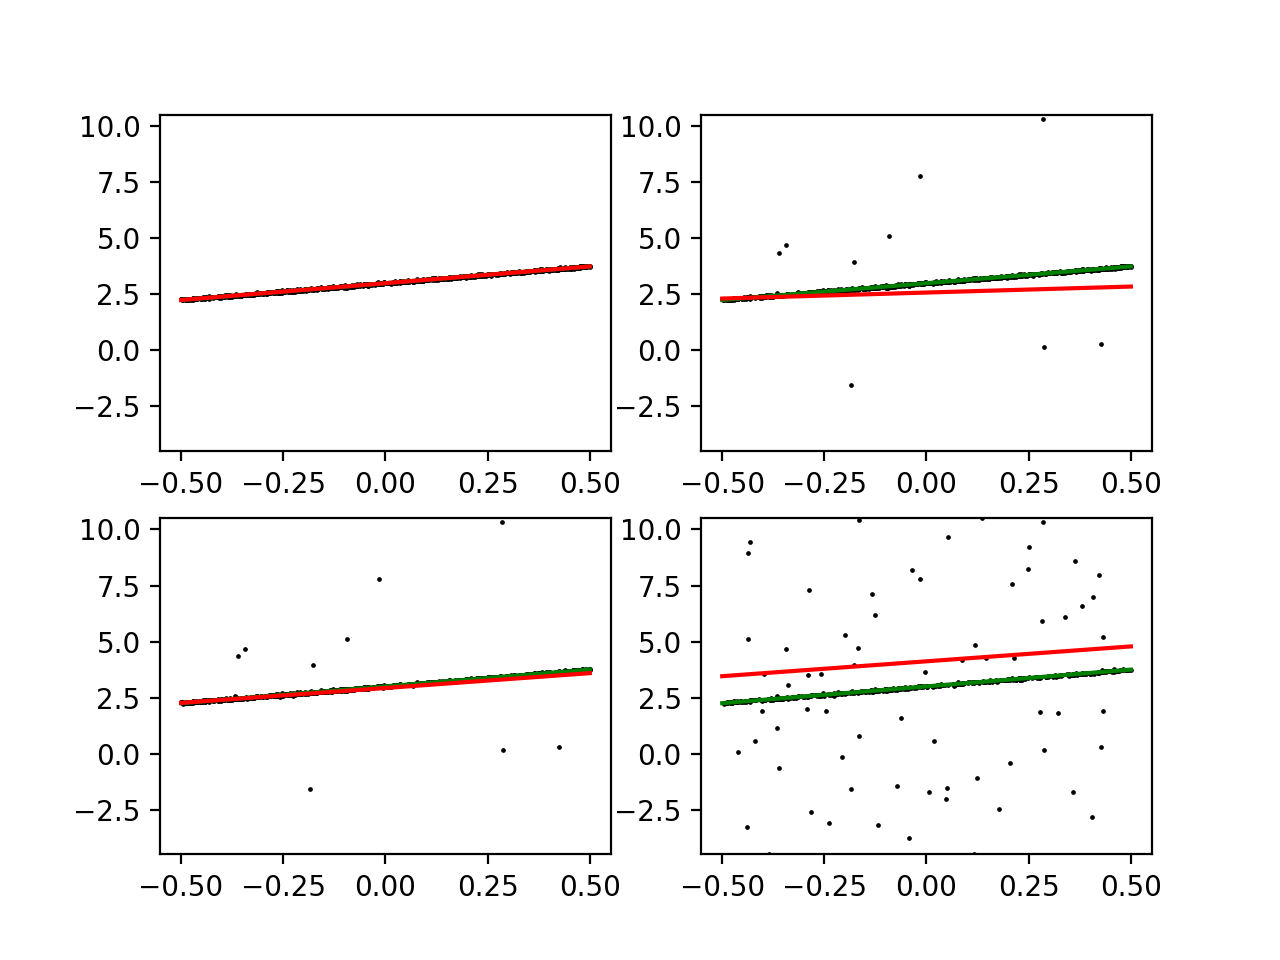
\includegraphics[height=30em]{code/outputs/prob2a.png}
	  \caption{Iterative Fitting}
\end{figure*}
\\
The number of iterations determines the fitting performance. For same number of outliers, the more iterations the better fitting performance, the less errors; for the same number of iterations, the more outliers the more errors.

\newpage
\spart{b}
RANSAC
\begin{figure*}[h!]
  \centering
	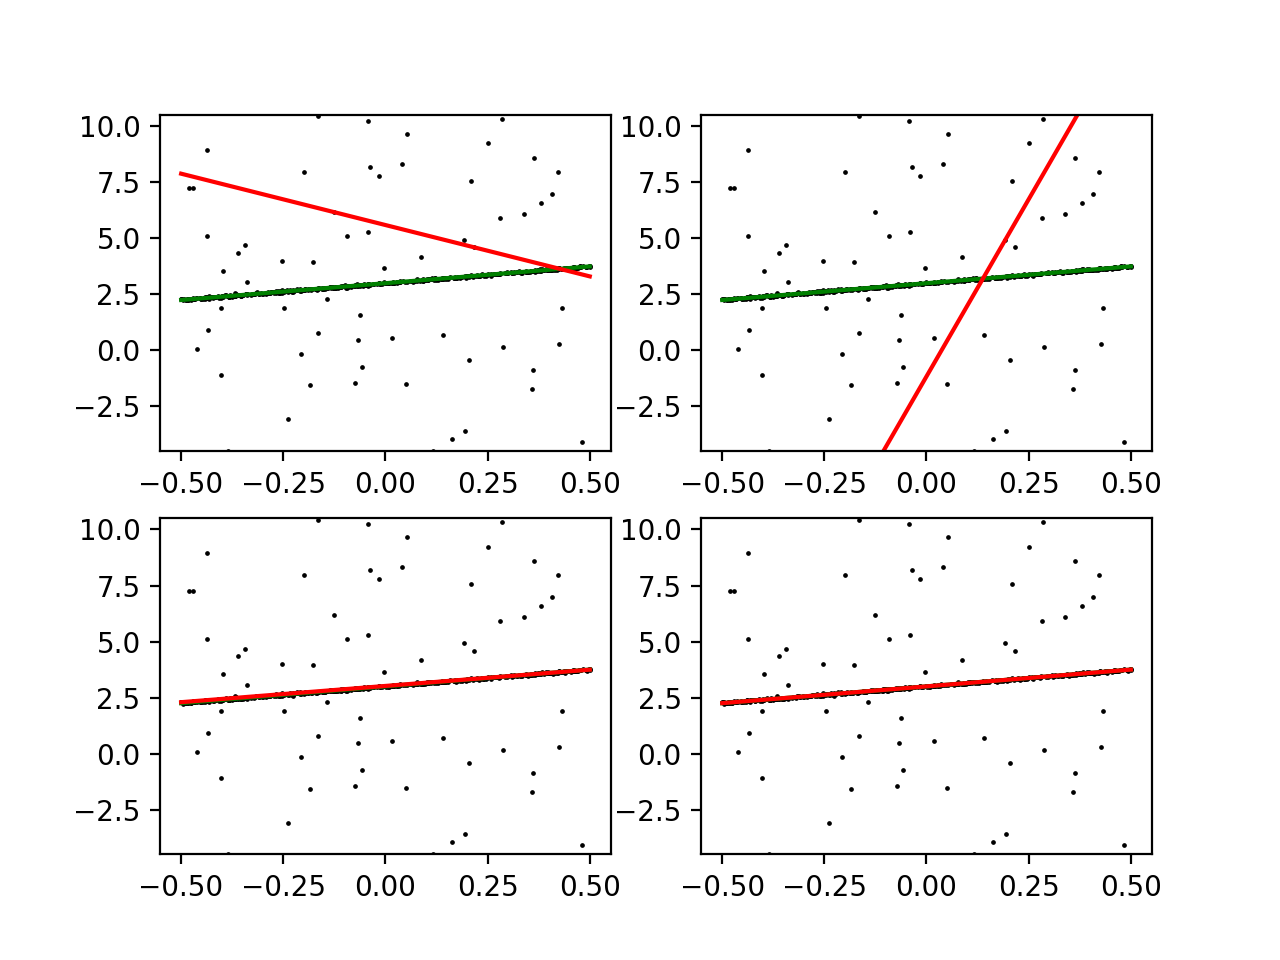
\includegraphics[height=30em]{code/outputs/prob2b.png}
	  \caption{RANSAC}
\end{figure*}
\\
The number of samples and runs determines the fitting performance. The more samples and runs, the better the performance is. The number of runs has more impact on the fitting performance, because when the number of runs is big enough, the performance is good enough no matter how many samples.

\solution{3}
\spart{a}
Assume there is a point $\left(x, y, z\right)$ in the real world. So, for camera 1, the expression from $\left(x, y, z\right)$ to $\left(x_1, y_1\right)$ is following:

\begin{equation}
	\left[
		\begin{array}{c}
		x_1 \\ y_1 \\ 1
		\end{array}
	\right] 
	\sim
	\left[
		\begin{array}{ccc}
		f_1 & 0 & W/2\\
		0 & f_1 & H/2\\
		0 & 0 & 1
		\end{array}
	\right]
	\left[
		\begin{array}{cccc}
		1 & 0 & 0 & 0\\
		0 & 1 & 0 & 0\\
		0 & 0 & 1 & 0
		\end{array}
	\right]
	\left[
		\begin{array}{c}
		x\\
		y\\
		z\\
		1
		\end{array}
	\right]
\end{equation}
\\The expression from  $\left(x, y, z\right)$ to $\left(x_2, y_2\right)$ is following:
\begin{equation}
	\left[
		\begin{array}{c}
		x_2 \\ y_2 \\ 1
		\end{array}
	\right] 
	\sim
	\left[
		\begin{array}{ccc}
		f_2 & 0 & W/2\\
		0 & f_2 & H/2\\
		0 & 0 & 1
		\end{array}
	\right]
	\left[
		\begin{array}{cccc}
		1 & 0 & 0 & 0\\
		0 & 1 & 0 & 0\\
		0 & 0 & 1 & 0
		\end{array}
	\right]
	\left[
		\begin{array}{c}
		x\\
		y\\
		z\\
		1
		\end{array}
	\right]
\end{equation}
\\So, we can get the following expression:
\begin{equation}
	\left[
		\begin{array}{cccc}
		1 & 0 & 0 & 0\\
		0 & 1 & 0 & 0\\
		0 & 0 & 1 & 0
		\end{array}
	\right]
	\left[
		\begin{array}{c}
		x\\
		y\\
		z\\
		1
		\end{array}
	\right]
	=
	\left[
		\begin{array}{ccc}
		\frac{1}{f_1} & 0 & \frac{-W/2}{f_1}\\
		0 & \frac{1}{f_1} & \frac{-H/2}{f_1}\\
		0 & 0 & 1\\
		\end{array}
	\right]	
	\left[
		\begin{array}{c}
		x_1\\
		y_1\\
		1
		\end{array}
	\right]
\end{equation}

\begin{equation}
	\left[
		\begin{array}{c}
		x_2 \\ y_2 \\ 1
		\end{array}
	\right] 
	\sim
	\left[
		\begin{array}{ccc}
		f_2 & 0 & W/2\\
		0 & f_2 & H/2\\
		0 & 0 & 1
		\end{array}
	\right]
	\left[
		\begin{array}{ccc}
		\frac{1}{f_1} & 0 & \frac{-W/2}{f_1}\\
		0 & \frac{1}{f_1} & \frac{-H/2}{f_1}\\
		0 & 0 & 1\\
		\end{array}
	\right]	
	\left[
		\begin{array}{c}
		x_1\\
		y_1\\
		1
		\end{array}
	\right]
	=
	\left[
		\begin{array}{ccc}
		\frac{f_2}{f_1} & 0 & \left(1 - \frac{f_2}{f_1}\right)\frac{W}{2}\\
		0 & \frac{f_2}{f_1} & \left(1 - \frac{f_2}{f_1}\right)\frac{H}{2}\\
		0 & 0 & 1\\
		\end{array}
	\right]	
	\left[
		\begin{array}{c}
		x_1\\
		y_1\\
		1
		\end{array}
	\right]
\end{equation}

\spart{b}
Assume all the points in the 3D world on a plane, set $Z = 0$, and assume rotation, translation and extrinsic matrices for two camera are respectively $R_1, t_1, K_1 and R_2, R_2, t_2, K_2$, and points in this plane of 3D world is $[X, Y, 0, 1]^T$, $[X_1, Y_1, 1]^T$ and $[X_2, Y_2, 1]^T$ are points in camera 1 and 2, so we can get following expressions:

\begin{align}
	\left[
		\begin{array}{c}
		X_1 \\ Y_1 \\ 1
		\end{array}
	\right] 
	\sim
	\left[
		\begin{array}{c}
		K_1
		\end{array}
	\right]
	\left[
		\begin{array}{cc}
		R_1 & t_1\\
		0^T & 1\\
		\end{array}
	\right]
	\left[
		\begin{array}{c}
		X\\
		Y\\
		0\\
		1
		\end{array}
	\right]
\end{align}

\begin{equation}
	\left[
		\begin{array}{c}
		X_2 \\ Y_2 \\ 1
		\end{array}
	\right] 
	\sim
	\left[
		\begin{array}{c}
		K_2
		\end{array}
	\right]
	\left[
		\begin{array}{cc}
		R_2 & t_2\\
		0^T & 1\\
		\end{array}
	\right]
	\left[
		\begin{array}{c}
		X\\
		Y\\
		0\\
		1
		\end{array}
	\right]
\end{equation}
\\These expressions can be shown as the following:
\begin{equation}
	\left[
		\begin{array}{c}
		X_1 \\ Y_1 \\ 1
		\end{array}
	\right] 
	\sim
	H_1
	\left[
		\begin{array}{c}
		X\\
		Y\\
		0\\
		1
		\end{array}
	\right]
\end{equation}

\begin{equation}
	\left[
		\begin{array}{c}
		X_2 \\ Y_2 \\ 1
		\end{array}
	\right] 
	\sim
	H_2
	\left[
		\begin{array}{c}
		X\\
		Y\\
		0\\
		1
		\end{array}
	\right]
\end{equation}
\\So, the expression for projected homogeneous co-ordinates in one camera in terms of those in another is:
\begin{equation}
	\left[
		\begin{array}{c}
		X_1 \\ Y_1 \\ 1
		\end{array}
	\right] 
	\sim
	H_1H^{-1}_2
	\left[
		\begin{array}{c}
		X_2 \\ Y_2 \\ 1
		\end{array}
	\right] 
\end{equation}



\solution{4}
\spart{b} Splice one image into another
\begin{figure*}[h!]
  \centering
	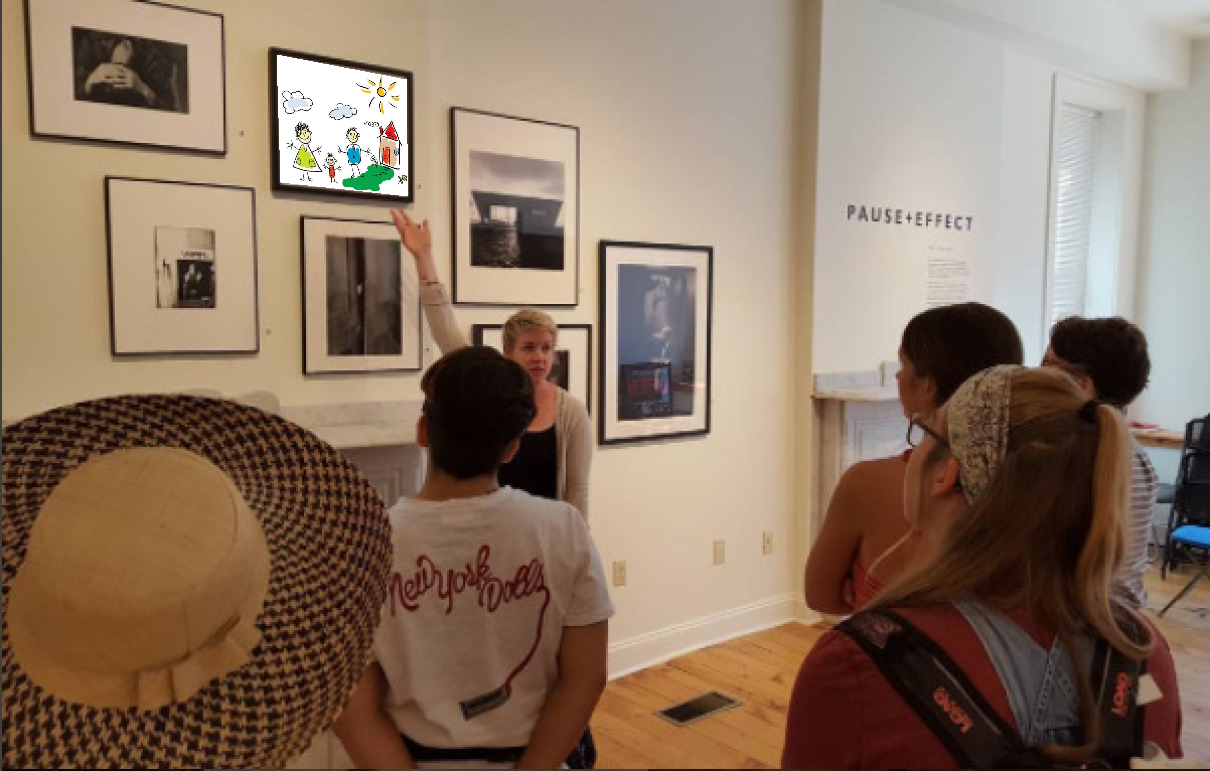
\includegraphics[height=30em]{code/outputs/prob4.png}
	  \caption{Spliced Image}
\end{figure*}

\solution{5}
\spart{b} Disparity Map
\begin{figure*}[h!]
  \centering
	
\includegraphics[height=16em]{code/outputs/prob5.png}
	  \caption{Disparity Map}
\end{figure*}


\info

This problem set took approximately 25 hours of effort.


I discussed this problem set with:
\begin{itemize}
\item Sijia Wang
\item Chunyuan Li
\item Jiarui Xing
\end{itemize}


% Note that you might have to escape some special symbols in URLS like \_
I also got hints from the following sources:
\begin{itemize}
\item lecture ppts
\end{itemize}

\end{document}
